\documentclass{article}
\usepackage{amsmath}
\usepackage{amsfonts}
\usepackage{amssymb}
\usepackage{graphicx}
\usepackage{tikz}
\usepackage{pgfplots}
\pgfplotsset{compat=1.18}
\begin{document}

\section{TikZ Diagrams ExamplesThis document demonstrates various TikZ diagrams that can be rendered in Overleaf. Each section shows different types of diagrams created using React components.

}

\section{Geometric ShapesThis section demonstrates basic TikZ geometric shapes.

\begin{figure}[h]
\centering
\begin{tikzpicture}[scale=1]
\draw[step=1cm] (0,0) grid (6,6);
\drawfill=blue!20, draw=blue (2,2) circle (1cm);
\drawfill=red!20, draw=red (4,4) rectangle (5.5,5);
\drawthick, green (1,1) -- (5,5);
\draw->, thick, purple (1,5) -- (5,1);
\nodeabove at (2,3.5) {Circle};
\nodeabove at (4.75,4.5) {Rectangle};
\nodeabove at (3,3) {Line};
\nodebelow at (3,3) {Arrow};

\end{tikzpicture}
\end{figure}

}

\section{Flowchart ExampleThis section shows a simple flowchart created with TikZ.

\begin{figure}[h]
\centering
\begin{tikzpicture}[scale=1]
\node[circle, draw] (0,0) {Start};
\node[rectangle, draw] (0,-2) {Process};
\node[rectangle, draw] (0,-4) {Decision};
\node[rectangle, draw] (3,-4) {Yes};
\node[rectangle, draw] (-3,-4) {No};
\node[circle, draw] (0,-6) {End};
\draw-> (0,-0.5) -- (0,-1.5);
\draw-> (0,-2.5) -- (0,-3.5);
\draw-> (0.5,-4) -- (2.5,-4);
\draw-> (-0.5,-4) -- (-2.5,-4);
\draw-> (0,-4.5) -- (0,-5.5);

\end{tikzpicture}
\end{figure}

}

\section{Mathematical DiagramThis section demonstrates a mathematical diagram with axes and functions.

\begin{figure}[h]
\centering
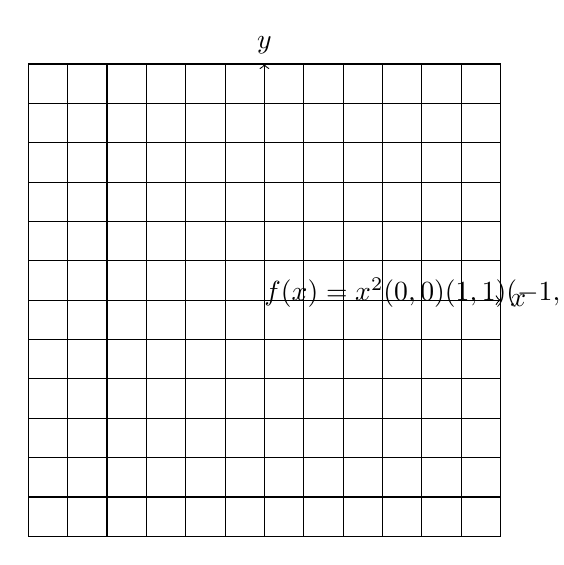
\begin{tikzpicture}[scale=1]
\draw[->] (-3,0) -- (3,0) node[right] {$x$};
\draw[->] (0,-3) -- (0,3) node[above] {$y$};
\draw[step=0.5cm] (-3,-3) grid (3,3);
\drawthick, blue (-2,4) -- (-1.5,2.25);
\drawthick, blue (-1.5,2.25) -- (-1,1);
\drawthick, blue (-1,1) -- (-0.5,0.25);
\drawthick, blue (-0.5,0.25) -- (0,0);
\drawthick, blue (0,0) -- (0.5,0.25);
\drawthick, blue (0.5,0.25) -- (1,1);
\drawthick, blue (1,1) -- (1.5,2.25);
\drawthick, blue (1.5,2.25) -- (2,4);
\drawfill=red (0,0) circle (0.05cm);
\drawfill=red (1,1) circle (0.05cm);
\drawfill=red (-1,1) circle (0.05cm);
\nodeblue at (2.5,3.5) {$f(x) = x^2$};
\nodered at (0.2,0.2) {$(0,0)$};
\nodered at (1.2,1.2) {$(1,1)$};
\nodered at (-1.2,1.2) {$(-1,1)$};

\end{tikzpicture}
\end{figure}

}

\section{Simple Circuit DiagramThis section shows a simple electrical circuit diagram.

\begin{figure}[h]
\centering
\begin{tikzpicture}[scale=1]
\drawthick (0,0) -- (0,1);
\drawthick (0.5,0) -- (0.5,1);
\drawthick (0,0.5) -- (0.5,0.5);
\drawthick (1,0.5) -- (1.5,0.5);
\drawthick (1.5,0.5) -- (1.5,0.3);
\drawthick (1.5,0.3) -- (2,0.3);
\drawthick (2,0.3) -- (2,0.5);
\drawthick (2,0.5) -- (2.5,0.5);
\drawfill=yellow!20, draw=black (3,0.5) circle (0.3cm);
\drawthick (2.5,0.5) -- (2.7,0.5);
\drawthick (3.3,0.5) -- (3.5,0.5);
\drawthick (3.5,0.5) -- (4,0.5);
\drawthick (4,0.5) -- (4,0);
\drawthick (4,0) -- (0,0);
\nodeabove at (0.25,1.5) {Battery};
\nodeabove at (1.75,1.5) {Resistor};
\nodeabove at (3,1.5) {LED};

\end{tikzpicture}
\end{figure}

}



\end{document}